\documentclass[aspectratio=169, 12pt]{beamer}

\usepackage[utf8]{inputenc}
\usepackage[T1]{fontenc}
\usepackage[spanish]{babel}
\usepackage{amsmath, amssymb}
\usepackage{booktabs}
\usepackage{array}
\usepackage{graphicx}
\usepackage{xcolor}
\usepackage{tikz}
\usetikzlibrary{arrows.meta, shapes.geometric, positioning, calc}
\usepackage{listings}
\usepackage{microtype}
\usepackage{enumitem}

\usepackage[sfdefault, light]{FiraSans}
\usepackage[lining]{FiraMono}
\renewcommand{\familydefault}{\sfdefault}

\usetheme[progressbar=frametitle, numbering=fraction, block=fill]{metropolis}

\definecolor{NavyBg}    {RGB}{13,  18,  38}
\definecolor{NavyFrame} {RGB}{20,  28,  60}
\definecolor{Cian}      {RGB}{0,  188, 212}
\definecolor{Verde}     {RGB}{0,  230, 118}
\definecolor{BlancoCool}{RGB}{220,230,255}
\definecolor{GrisAzul}  {RGB}{140,160,210}
\definecolor{CodeBg}    {RGB}{28,  36,  70}
\definecolor{AlertRed}  {RGB}{255,  82,  82}

\setbeamercolor{normal text}         {fg=BlancoCool, bg=NavyBg}
\setbeamercolor{background canvas}   {bg=NavyBg}
\setbeamercolor{frametitle}          {fg=Verde, bg=NavyFrame}
\setbeamercolor{progress bar}        {fg=Cian, bg=NavyFrame}
\setbeamercolor{title separator}     {fg=Cian}
\setbeamercolor{structure}           {fg=Cian}
\setbeamercolor{alerted text}        {fg=Verde}
\setbeamercolor{block title}         {fg=Verde, bg=CodeBg}
\setbeamercolor{block body}          {fg=BlancoCool, bg=NavyFrame}
\setbeamercolor{block title example} {fg=Cian, bg=CodeBg}
\setbeamercolor{block body example}  {fg=BlancoCool, bg=NavyFrame}
\setbeamercolor{itemize item}        {fg=Verde}
\setbeamercolor{itemize subitem}     {fg=Cian}
\setbeamercolor{enumerate item}      {fg=Verde}
\setbeamercolor{title}               {fg=Verde}
\setbeamercolor{subtitle}            {fg=Cian}
\setbeamercolor{author}              {fg=GrisAzul}
\setbeamercolor{date}                {fg=GrisAzul}
\setbeamercolor{section in toc}      {fg=BlancoCool}

\setbeamerfont{frametitle}{size=\large, series=\bfseries}
\setbeamerfont{title}     {size=\Large, series=\bfseries}
\setbeamerfont{block title}{size=\small, series=\bfseries}

\lstset{
  language        = C++,
  basicstyle      = \ttfamily\tiny\color{BlancoCool},
  keywordstyle    = \color{Cian}\bfseries,
  commentstyle    = \color{GrisAzul}\itshape,
  stringstyle     = \color{Verde},
  numberstyle     = \tiny\color{GrisAzul},
  backgroundcolor = \color{CodeBg},
  frame           = single,
  rulecolor       = \color{Cian!40},
  numbers         = left,
  numbersep       = 4pt,
  breaklines      = true,
  showstringspaces= false,
  tabsize         = 2,
  xleftmargin     = 1.2em,
  framexleftmargin= 0.8em,
  morekeywords    = {vector, string, size_t, mt19937},
}

\newcommand{\acento}[1]{\textcolor{Verde}{\textbf{#1}}}
\newcommand{\acentob}[1]{\textcolor{Cian}{#1}}
\newcommand{\gris}[1]{\textcolor{GrisAzul}{#1}}

\title{EVCSPP: Optimización Evolutiva de\\Estaciones de Carga para VE}
\subtitle{Presentación Final}
\author{Matias Lara Plaza}
\institute{Inteligencia Artificial $\cdot$ 2026-1}
\date{Junio 2026}

\begin{document}

% =====  1. PORTADA  =====
\maketitle

% =====  2. AGENDA  =====
\begin{frame}{Contenido}
  \setbeamertemplate{section in toc}[sections numbered]
  \tableofcontents
\end{frame}

% ============================================================
\section{El Problema}
% ============================================================

% =====  3. ENCUADRE MÍNIMO (comprimido de 3 slides a 1)  =====
\begin{frame}{Encuadre: el problema EVCSPP}
  \begin{columns}[T]
    \column{0.55\textwidth}
    \begin{itemize}
      \item \textbf{EVCSPP}: elegir \emph{qué nodos} de una red alojan estaciones de carga, minimizando el costo total de construcción.
      \item Formalmente \alert{NP-duro} \gris{[Lam et al., 2014]}: $2^n$ soluciones para $n$ ubicaciones candidatas.
    \end{itemize}
    \vspace{0.4em}
    \textbf{Función objetivo:}
    \[ \min \sum_{j=1}^{n} C_j \cdot x_j, \qquad x_j \in \{0,1\} \]
    \gris{\footnotesize $x_j = 1$: se construye estación en el nodo $j$; $C_j$ es su costo.}

    \column{0.43\textwidth}
    \begin{block}{Sujeto a 4 restricciones}
      \begin{itemize}\footnotesize
        \item[\acento{R1}] Accesibilidad
        \item[\acento{R2}] Demanda (anillo $[\alpha R,\,R]$)
        \item[\acento{R3}] Cobertura urbana
        \item[\acento{R4}] Zonas remotas
      \end{itemize}
    \end{block}
    \vspace{0.3em}
    \gris{\scriptsize El modelo y el manejo de las restricciones se detallan en la sección siguiente.}
  \end{columns}
\end{frame}

% ============================================================
\section{Propuesta}
% ============================================================

% =====  4. REPRESENTACIÓN (reusada)  =====
\begin{frame}[fragile]{Representación: Cromosoma Binario}
  \begin{columns}[T]
    \column{0.47\textwidth}
    \textbf{Una solución = vector binario de longitud $n$:}
    \vspace{0.15em}
    \begin{center}
    \begin{tikzpicture}[scale=0.80]
      \foreach \i/\v/\col in {0/1/Verde,1/0/GrisAzul,2/0/GrisAzul,3/1/Verde,4/1/Verde,5/0/GrisAzul}{
        \node[draw=Cian!60,fill=CodeBg,minimum width=0.70cm,minimum height=0.65cm,text=\col,font=\small\bfseries]
          at (\i*0.83,0) {\v};
        \node[font=\tiny,GrisAzul] at (\i*0.83,-0.46){$j{=}\i$};
      }
      \draw[<-,Verde,thick] (0,0.38)--++(0,0.32) node[above,font=\tiny,Verde]{construir};
    \end{tikzpicture}
    \end{center}
    \vspace{0.1em}
    \begin{itemize}
      \item Longitud = \texttt{n\_nodes} (de la instancia)
      \item Homogéneo, sin orden implícito
      \item Compatible con GA binario estándar
    \end{itemize}

    \column{0.51\textwidth}
    \textbf{Implementación (\texttt{Solution.h}):}
    \begin{lstlisting}
class Solution {
public:
  // Cromosoma: 1=construir, 0=no
  vector<int> chromosome;

  const Instance* instance;

  double cost;    // costo real
  double penalty; // suma penalidades
  double fitness; // cost + penalty

  Solution(const Instance* inst);
  void evaluate();            // calcula fitness
  void randomize(mt19937&);   // sol. inicial
};
    \end{lstlisting}
  \end{columns}
\end{frame}

% =====  5. RESTRICCIONES (comprimido de 3 slides a 1)  =====
\begin{frame}{Manejo de Restricciones: Penalidades}
  \begin{columns}[T]
    \column{0.46\textwidth}
    \textbf{Estrategia:} restricciones $\rightarrow$ penalidades aditivas
    {\setlength\abovedisplayskip{3pt}\setlength\belowdisplayskip{3pt}
    \[
      \text{fitness} =
        \underbrace{\sum_{j:\,x_j=1}C_j}_{\text{costo base}}
        + \underbrace{\lambda\sum_k\delta_k}_{\text{penalidades}}
    \]
    }
    Con $\lambda = 10^9 \gg$ cualquier costo real.
    \vspace{0.3em}
    \begin{block}{Por qué funciona}
      \footnotesize Toda solución infactible queda con fitness $\gg$ que cualquier factible, sin necesidad de descartarla. R2 penaliza proporcional al déficit.
    \end{block}

    \column{0.52\textwidth}
    \textbf{Las 4 restricciones:}
    \vspace{0.3em}
    \begin{itemize}\footnotesize
      \item[\acento{R1}] \textbf{Accesibilidad:} $\;x_i + x_j \geq 1 \quad \forall(i,j)\in\bar{E}$
      \vspace{0.25em}
      \item[\acento{R2}] \textbf{Demanda:} $\;\sum_{i\in V_j^{\alpha R}} f_i\,x_i \geq D_j$ \\
        \gris{\scriptsize anillo $V_j^{\alpha R}=\{i : \alpha R \le d(i,j) \le R\}$}
      \vspace{0.25em}
      \item[\acento{R3}] \textbf{Cobertura urbana:} $\;\sum_{j} s_j\,x_j \geq \textit{CityArea}$
      \vspace{0.25em}
      \item[\acento{R4}] \textbf{Zonas remotas:} $\;\sum_{j\in T} x_j \geq 1$
    \end{itemize}
  \end{columns}
\end{frame}

% =====  6. FLUJO DEL GA  =====
\begin{frame}{El Algoritmo Genético: Flujo Completo}
  \begin{columns}[T]
    \column{0.52\textwidth}
    \begin{block}{Parámetros implementados}
      \footnotesize
      \begin{tabular}{@{}ll@{}}
        \acentob{pop\_size}       & eje del barrido $\{10,...,200\}$ \\
        \acentob{crossover\_rate} & 0.9 (uniforme) \\
        \acentob{mutation\_rate}  & $1/n$ por gen \\
        \acentob{criterio parada} & estancamiento \\
                                   & (\texttt{patience}$=200$) o \\
                                   & \texttt{max\_gen}$=4000$ \\
      \end{tabular}
    \end{block}
    \vspace{0.5em}
    \begin{block}{Por qué ese criterio de parada}
      \scriptsize El estancamiento corta apenas el GA deja de mejorar (ahorra cómputo); el tope \texttt{max\_gen} evita ciclos sin fin cuando nunca se alcanza factibilidad ($\alpha$ alto).
    \end{block}

    \column{0.45\textwidth}
    \begin{center}
    \begin{tikzpicture}[
      scale=0.78,
      caja/.style ={draw=Cian!60,fill=CodeBg,text=BlancoCool,
                    rounded corners=3pt,minimum width=4.3cm,
                    minimum height=0.52cm,font=\scriptsize,align=center},
      cajae/.style={draw=Verde,fill=Verde!60,text=NavyBg,
                    rounded corners=3pt,minimum width=4.3cm,
                    minimum height=0.52cm,font=\scriptsize\bfseries,align=center},
      fl/.style   ={-Stealth,GrisAzul,thick}]
      \node[caja]  (ini)   at (0, 5.0){Poblar con \texttt{randomize()}};
      \node[caja]  (eval)  at (0, 4.1){Evaluar fitness de la población};
      \node[cajae] (elit)  at (0, 3.2){Elitismo: copiar el mejor directo};
      \node[caja]  (sel)   at (0, 2.3){Selección por Ruleta ($\times$2)};
      \node[caja]  (cross) at (0, 1.4){Cruce Uniforme ($p_c = 0.9$)};
      \node[caja]  (mut)   at (0, 0.5){Mutación Bit-flip ($p_m = 1/n$)};
      \node[caja]  (rep)   at (0,-0.4){Reemplazar generación};
      \foreach \a/\b in {ini/eval,eval/elit,elit/sel,sel/cross,cross/mut,mut/rep}
        \draw[fl] (\a)--(\b);
      \draw[-Stealth,Cian,thick]
        (rep.east)--++(0.35,0)--++(0,4.6)
        node[pos=0.5,right=2pt,font=\tiny,Cian]{patience/max\_gen}
        --(eval.east);
    \end{tikzpicture}
    \end{center}
  \end{columns}
\end{frame}

% =====  7. OPERADORES (comprimido: 3 movimientos + justificación en 1)  =====
\begin{frame}{Operadores del GA y su justificación}
  \footnotesize
  \begin{columns}[T]
    \column{0.5\textwidth}
    \acento{Selección: ruleta invertida}
    {\setlength\abovedisplayskip{2pt}\setlength\belowdisplayskip{2pt}
    \[ \tilde{f}_i = (\max_k f_k - f_i) + 1 \]}
    \gris{Adaptada a minimización. El \texttt{+1} impide que el mejor quede con probabilidad nula. Presión selectiva sin monopolizar.}
    \vspace{0.5em}

    \acento{Cruce uniforme} ($p_c$)\\
    \gris{Cada gen hereda de un padre con $p=0.5$, de forma independiente. Máxima mezcla y sin sesgo posicional (a diferencia del cruce de 1 punto): exploración amplia.}

    \column{0.5\textwidth}
    \acento{Mutación bit-flip} ($p_m = 1/n$)\\
    \gris{Cada gen se niega con probabilidad $p_m$. Perturbación mínima para escapar de óptimos locales sin destruir buenas soluciones.}
    \vspace{0.5em}

    \acento{Elitismo (1-best)}\\
    \gris{El mejor de cada generación pasa intacto a la siguiente: el fitness global nunca empeora.}
    \vspace{0.5em}

    \acento{Penalidad} $\lambda = 10^9$\\
    \gris{$\lambda \gg$ cualquier costo real: las soluciones infactibles son siempre peores que las factibles.}
  \end{columns}
  \vspace{0.4em}
  \begin{block}{Orden en cada generación}
    \footnotesize Elitismo $\rightarrow$ Ruleta $\times 2$ $\rightarrow$ Cruce $\rightarrow$ Bit-flip $\rightarrow$ Evaluar
  \end{block}
\end{frame}

% ============================================================
\section{Recomendaciones de Estado de Avance}
% ============================================================

% =====  8. RECOMENDACIONES DE ESTADO DE AVANCE  =====
\begin{frame}{Recomendaciones de Estado de Avance}
  \footnotesize\gris{El ayudante entregó 2 recomendaciones en la Presentación de Estado de Avance. Cada una se abordó con un experimento dedicado (siguientes diapositivas).}
  \vspace{0.6em}
  \begin{columns}[T]
    \column{0.48\textwidth}
    \begin{block}{\acento{1.} Tamaño de población}
      \footnotesize
      \textbf{Observación:} \texttt{pop\_size=50} se usaba sin respaldo experimental.
      \vspace{0.4em}

      \textbf{Qué hicimos:} barrido dedicado de \texttt{pop\_size} $\in\{10,20,50,100,200\}$, midiendo costo final y esfuerzo (evaluaciones).
      \vspace{0.6em}

      \acentob{$\rightarrow$ Experimento 1}
    \end{block}

    \column{0.48\textwidth}
    \begin{block}{\acento{2.} Visualización y $\alpha$}
      \footnotesize
      \textbf{Observación:} faltaba ver \emph{dónde} construye el GA y el efecto del parámetro $\alpha$ del problema.
      \vspace{0.4em}

      \textbf{Qué hicimos:} barrido de $\alpha \in \{0,\,0.05,\,0.10,\,0.15,\,0.20\}$ y mapa de la mejor solución factible encontrada.
      \vspace{0.6em}

      \acentob{$\rightarrow$ Experimento 2}
    \end{block}
  \end{columns}
\end{frame}

% ============================================================
\section{Experimentos y Resultados}
% ============================================================

% =====  9. DISEÑO EXPERIMENTAL  =====
\begin{frame}{Diseño Experimental}
  \begin{columns}[T]
    \column{0.54\textwidth}
    \textbf{\footnotesize Barrido de 2 ejes:} $\alpha$ (problema) $\times$ \texttt{pop\_size} (algoritmo).
    \vspace{0.2em}
    \begin{center}
    \begin{tikzpicture}[font=\tiny]
      \node[GrisAzul] at (3.05,0.95) {\texttt{pop\_size}};
      \foreach \j/\poplbl in {0/10,1/20,2/50,3/100,4/200}{
        \node[GrisAzul] at (\j*0.95+1.15, 0.5) {\poplbl};
      }
      \foreach \i/\alphalbl in {0/0,1/0.05,2/0.10,3/0.15,4/0.20}{
        \node[GrisAzul,anchor=east] at (0.75,-\i*0.6) {$\alpha{=}\alphalbl$};
        \foreach \j in {0,...,4}{
          \node[draw=Cian!50,fill=CodeBg,minimum width=0.8cm,minimum height=0.48cm,text=BlancoCool]
            at (\j*0.95+1.15, -\i*0.6) {25};
        }
      }
    \end{tikzpicture}
    \end{center}
    \gris{\scriptsize Cada celda = 25 corridas (5 instancias $\times$ 5 semillas) $\Rightarrow$ \textbf{625 corridas} en total.}

    \column{0.43\textwidth}
    \scriptsize
    \begin{itemize}[itemsep=4pt,topsep=2pt,parsep=0pt,leftmargin=1.1em]
      \item \acento{Instancias:} 5 reales \texttt{S71--S75} ($n{=}100$); mismo mapa/costos, difieren en capacidad $f_i$.
      \item \acento{Réplicas:} 5 semillas/config. $\rightarrow$ media $\pm$ desv. estándar (robustez ante el azar del GA, no es eje).
      \item \acento{Fijos:} \texttt{crossover}$=0.9$, \texttt{mutation}$=1/n$ (principistas, no se barren).
      \item \acento{Término doble:} estancamiento (\texttt{patience}$=200$ si ya es factible) $+$ tope duro \texttt{max\_gen}$=4000$.
      \item \acento{Esfuerzo:} \texttt{evaluaciones}$=$pop$\times$gen\_alcanzado, moneda honesta e independiente del hardware.
    \end{itemize}
  \end{columns}
\end{frame}

% =====  10. EXPERIMENTO 1  =====
\begin{frame}{Experimento 1: Afinamiento del tamaño de población}
  \begin{columns}[T]
    \column{0.5\textwidth}
    \centering
    
\includegraphics[width=0.92\textwidth]{images/costo_vs_pop.png}\\[-0.2em]
    \scriptsize\gris{Costo final vs. \texttt{pop\_size}}

    \column{0.5\textwidth}
    \centering
    
\includegraphics[width=0.92\textwidth]{images/costo_y_esfuerzo_vs_pop.png}\\[-0.2em]
    \scriptsize\gris{Costo y esfuerzo vs. \texttt{pop\_size}}
  \end{columns}
  \footnotesize
  \textbf{Hallazgo:} en $\alpha{=}0.10$ todas las corridas son factibles para todo \texttt{pop\_size}, pero el costo y el esfuerzo NO mejoran al crecer la población.\\[0.3em]
  \acento{\texttt{pop\_size}$=200$ vs.\ \texttt{pop\_size}$=10$: 1.97$\times$ más caro y 16.7$\times$ más esfuerzo.}\\[0.3em]
  \gris{$\Rightarrow$ el esfuerzo (evaluaciones), no el tamaño de la población, es la palanca real. \acentob{Óptimo práctico: \texttt{pop\_size}$\in[10,20]$.}}
\end{frame}

% =====  11. EXPERIMENTO 2  =====
\begin{frame}{Experimento 2: Efecto de $\alpha$ en el comportamiento de la solución}
  \begin{columns}[T]
    \column{0.5\textwidth}
    \centering
    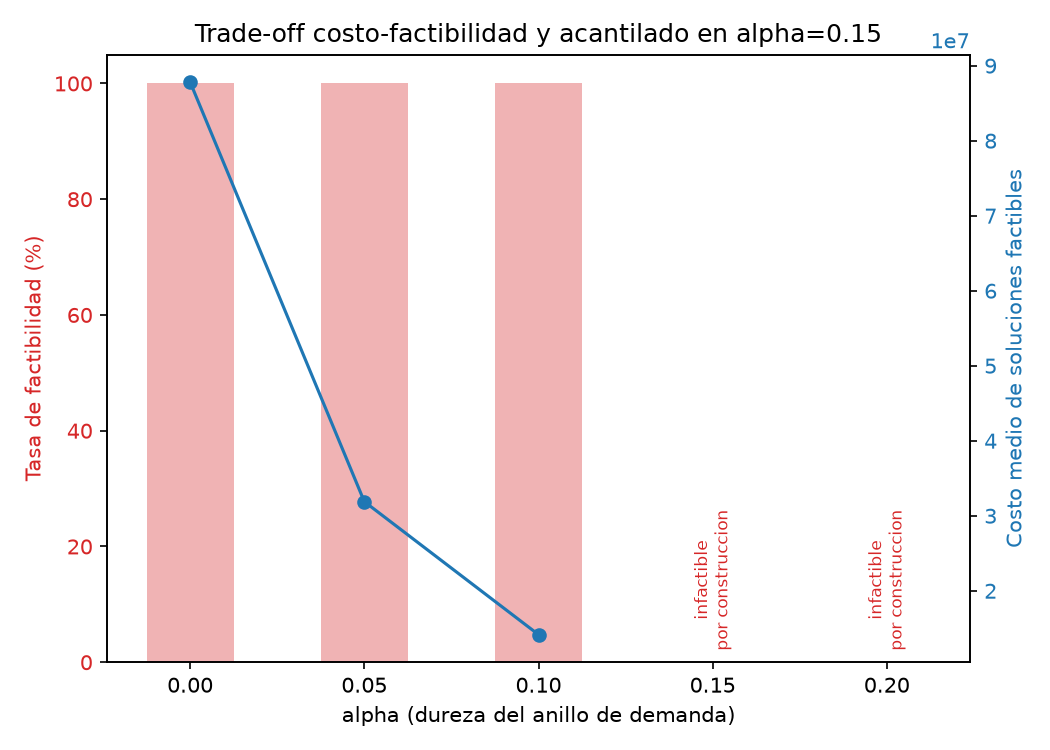
\includegraphics[width=0.85\textwidth]{images/factibilidad_vs_alpha.png}\\[-0.3em]
    \scriptsize\gris{Costo medio y factibilidad según $\alpha$ (625 corridas)}

    \column{0.5\textwidth}
    \centering
    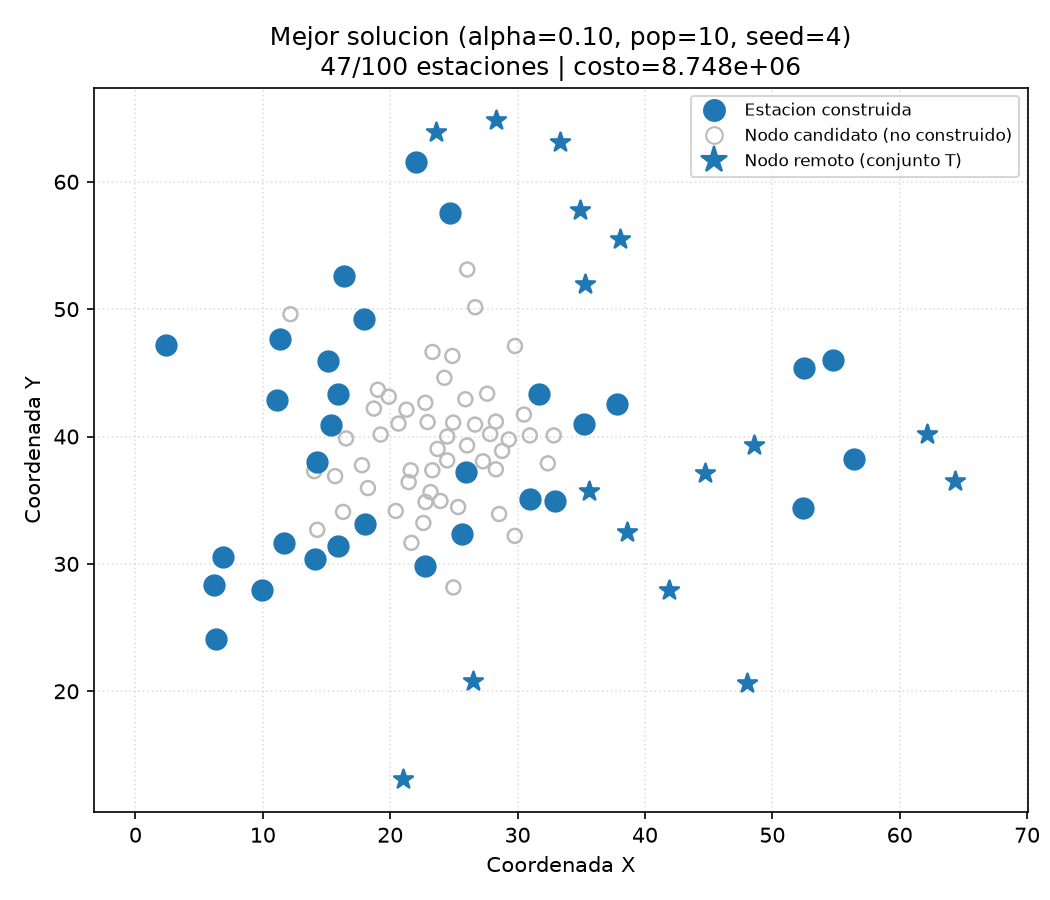
\includegraphics[width=0.85\textwidth]{images/mapa_solucion.png}\\[-0.3em]
    \scriptsize\gris{Solución representativa ($\alpha{=}0.10$): $47/100$ estaciones, costo $8.75\times 10^6$}
  \end{columns}
  \scriptsize
  \textbf{Hallazgo:} al crecer $\alpha$ el anillo de demanda excluye estaciones cercanas y la red se vuelve más dispersa: $\alpha{=}0\!\to\!99/100$ (87.8M), $\alpha{=}0.05\!\to\!68/100$ (31.9M), $\alpha{=}0.10\!\to\!48/100$ (14.2M), todas 100\% factibles. \acento{Límite: $\alpha\geq 0.15$ es infactible por construcción (0/125)}, no por debilidad del GA.
\end{frame}

% =====  12. APORTES DE LA IMPLEMENTACIÓN  =====
\begin{frame}{Aportes de la Implementación}
  \begin{columns}[T]
    \column{0.46\textwidth}
    \footnotesize
    \textbf{1. Detectar la frontera de factibilidad evita cómputo en vano.}\\[0.3em]
    {\scriptsize Un chequeo analítico previo (¿la solución todo-unos satisface R2?) descarta instancias infactibles por construcción ($\alpha\geq 0.15$) sin gastar una sola generación del GA.}
    \vspace{0.5em}
    \begin{center}
    \begin{tikzpicture}[font=\tiny]
      \node[draw=Cian!50,fill=CodeBg,text=BlancoCool,rounded corners,minimum width=2.6cm,minimum height=0.5cm] (inst) {Instancia $+\ \alpha$};
      \node[draw=Cian!50,fill=CodeBg,text=BlancoCool,rounded corners,minimum width=2.6cm,minimum height=0.5cm,below=0.45cm of inst] (check) {¿Todo-unos satisface R2?};
      \node[draw=AlertRed!70,fill=CodeBg,text=BlancoCool,rounded corners,minimum width=2.1cm,minimum height=0.5cm,below left=0.55cm and -0.4cm of check] (no) {Descartar};
      \node[draw=Verde!70,fill=CodeBg,text=BlancoCool,rounded corners,minimum width=2.1cm,minimum height=0.5cm,below right=0.55cm and -0.4cm of check] (si) {Correr GA};
      \draw[-{Stealth},GrisAzul] (inst) -- (check);
      \draw[-{Stealth},AlertRed] (check) -| node[above,pos=0.25,AlertRed]{No} (no);
      \draw[-{Stealth},Verde] (check) -| node[above,pos=0.25,Verde]{Sí} (si);
    \end{tikzpicture}
    \end{center}

    \column{0.5\textwidth}
    \footnotesize
    \textbf{2. Más población no es más calidad.}\\[0.2em]
    {\scriptsize A diferencia de la práctica habitual de escalar \texttt{pop\_size} para mejorar resultados, demostramos lo contrario: \acento{\texttt{pop\_size}$=200$ cuesta 1.97$\times$ más y gasta 16.7$\times$ más esfuerzo que \texttt{pop\_size}$=10$, sin mejorar el costo} (Experimento 1).}

    \vspace{1.6em}
    \textbf{3. Accesible sin hardware especializado.}\\[0.2em]
    {\scriptsize El mismo modelo que Ou et al. (2025) resuelven con \textit{digital quantum annealing} propietario, aquí se resuelve con un GA clásico en un notebook común. \gris{Sin comparación cuantitativa directa: instancias y costos propios, no coinciden con su Tabla IV.}}
  \end{columns}
\end{frame}

% ============================================================
\section{Conclusiones}
% ============================================================

% =====  13. CONCLUSIONES (modificada: 3 aspectos de la rúbrica)  =====
\begin{frame}{Conclusiones}
  \begin{enumerate}
    \item \acento{Dificultad del problema.}
      {\footnotesize NP-duro ($2^n$ soluciones). Además, con $\alpha \geq 0.15$ las instancias reales se vuelven \alert{infactibles por construcción}: el anillo de demanda R2 deja a varias zonas sin capacidad suficiente.}
      % TODO afinar con la frontera 0.11-0.14
    \vspace{0.4em}
    \item \acentob{Uso del algoritmo.}
      {\footnotesize El GA resuelve bien con $\alpha$ bajo (0 a 0.10). El \textbf{esfuerzo} (generaciones $\times$ población), y no el tamaño de la población, es la palanca de calidad: \acento{\texttt{pop\_size}$=200$ cuesta 1.97$\times$ más y gasta 16.7$\times$ más esfuerzo que \texttt{pop\_size}$=10$, sin mejorar el costo}.}
    \vspace{0.4em}
    \item \gris{Trabajo futuro.}
      {\footnotesize Afinar la frontera $\alpha \in [0.11, 0.14]$; comparación cuantitativa con el estado del arte; inicialización greedy frente a aleatoria.}
  \end{enumerate}
\end{frame}

% =====  14. REFERENCIAS (reusada)  =====
\begin{frame}{Referencias}
  \begin{enumerate}\footnotesize
    \item \textcolor{BlancoCool}{C.-H. Ou, C.-C. Cheng, C.-Y. Chen, K. Bhumkittipich, S. Romphochai.}
      \gris{``Solving Optimal EV Charging Station Placement Problem Using Digital Quantum Annealing.''}
      \textit{J. Comm. and Networks}, 27(4):252--263, \textbf{2025.}
      \hfill\acento{[Paper base]}

    \vspace{0.15em}
    \item \textcolor{BlancoCool}{A.~Y.~S. Lam, Y.-W. Leung, X. Chu.}
      \gris{``EV Charging Station Placement: Formulation, Complexity, and Solutions.''}
      \textit{IEEE Trans. Smart Grid}, 5(6):2846--2856, \textbf{2014.}
      \hfill\acentob{[Formulación]}

    \vspace{0.15em}
    \item \textcolor{BlancoCool}{H.~K. Demiryürek, B. Bozali, A. Ozturk.}
      \gris{``Optimal Placement and Cost Analysis of EV Charging Stations Using Metaheuristic Optimization.''}
      \textit{Applied Sciences}, 15(21), \textbf{2025.}

    \vspace{0.15em}
    \item \textcolor{BlancoCool}{S. Basu, M. Sharma, P.~S. Ghosh.}
      \gris{``Metaheuristic Applications on Discrete Facility Location Problems: A Survey.''}
      \textit{Opsearch}, 52(3):530--561, \textbf{2015.}
  \end{enumerate}

  \vspace{0.2em}
  \begin{center}
    \textcolor{Cian}{\rule{0.75\textwidth}{0.4pt}}\\[0.2em]
    \gris{\footnotesize Repositorio: \texttt{evcs-evolutionary-optimization} $\cdot$ Matias Lara Plaza $\cdot$ 2026}
  \end{center}
\end{frame}

% =====  15. CIERRE (portada repetida)  =====
\maketitle

\end{document}
